\chapter{Multi-Agent System with Multiple Group Modelling for Bird Flocking
	on GPU}
\label{ch:flocking}
\dictum[Gottfried Leibniz]{There are two kinds of truths: those of reasoning and those of fact. The truths of reasoning are necessary and their opposite is impossible; the truths of fact are contingent and their opposites are possible.}%
\vskip 1em

This chapter is adapted from \cite{rahmat:2016}.
%\section{Introduction}

\lettrine[lines=3,lhang=0.33,lraise=0,loversize=0.15]{T}{he} study of collective coherent motion of self-propelled biological organisms such as flocks of birds, schools of fish and swarms of insects has fascinated humans from ancient time. This kind of behaviour, often referred to as flocking, exists in nature at almost every
length scale of observation: from human crowds, mammalian herds, bird flocks,
fish schools to unicellular organisms such as amoebae and bacteria, individual
cells, and even at a microscopic level in the dynamics of acting and
tubular filaments and molecular motors. Despite the huge differences in the scales
of aggregations, the similarities in the patterns that such groups produce have
suggested that general principles may underlie collective motion.

An effective approach to study these collective behaviours is represented by
mathematical modelling and numerical simulation, as proven by numerous papers
published in this field that are related with both biology and computer
science (e.g., \cite{Schmickl}). In models that study simple motion principles of organisms like flocking, shoaling or phenomena based on random motion, organisms are treated like gas molecules and their motion is
Brownian combined with attraction/repulsion forces. Also ‘mean-field’ approaches, mainly carried out by adopting ordinary differential equation (ODE) models, might be useful to model some biological
swarm systems, whenever the assumption of a ‘well mixed’ distribution may be applicable.
However, organisms seldom move really randomly, nor are they just simple particles. They
pursue specific goals, aggregate or disperse in space, communicate and memorize. They can be characterized by specific physiological states (e.g. energy-level) and morphologies (size, weights, etc.).
These factors do not only affect their energetics, but may have prominently affect the behaviours
that they (choose to) perform. In addition, they frequently interact by direct and indirect
communication and they tend to memorize past effects. Eventually, also the environment
in which they operate is highly structured and this heterogeneity is also dynamic.
All these factors describe important discrepancies between biological life forms
and atoms or molecules. Thus, it is likely that models, which were originally derived from physics and chemistry, might not hold well
for biological swarm systems as soon as a certain level of abstraction has to be overcome.
In these cases, individual-based models or even multi-agent
models \cite{Ferber:1999,Woolridge:2001} might be a better choice.

In this paper we present the
\textsc{ACIADDRI}\footnote{ Meaning \textit{birds} in Calabrian language.} (\emph{\textbf{A}ggregate \textbf{C}ollection of \textbf{I}nteractive \textbf{A}gents using NVI\textbf{D}IA CU\textbf{D}A \textbf{R}eliable \textbf{I}nformatics}) multi-agent flocking model, besides an efficient GPGPU implementations on SIMT architectures. In particular, section \ref{sect:aciaddri}
formalizes the model and \ref{sect:gpuimplementation} the parallel
implementation using the CUDA framework.
Specifically, starting from Reynolds works \cite{Reynolds:1987}\cite{Reynolds:1999}\cite{Reynolds:2000} on bird flocking behaviour, \textsc{ACIADDRI} extends it by means of
additional features such as support for multi-species interaction, predator
avoidance, partially observable environment and birds flight constraints
(maximum thrust, stall and peak velocity, etc.). Section \ref{sect:gpuimplementation} reports experiments carried out on the
specific GPU hardware and by considering both aggregate motion of a huge number (up to tens of millions) of boids in a virtual
environment and other species or predators avoidance, significant performance
improvement in terms of speedup were obtained ( 
up to $ 500\times$), while
conclusions and future works are reported at the end of the paper.




\section{The ACIADDRI Model}
\label{sect:aciaddri}

This work is  based on flocking behaviour that was proposed by Craig W. Reynolds
in 1987 and extends it by adding both the support to coexistence and interaction
between different species, and the predator avoidance.
Reynolds was amongst the first to abstract this behaviour, in order to steer a swarm
of simulated birds which he called boids\cite{Reynolds}(contraction of birdoid).
Every boid has some limitations:
it has a strictly local knowledge of the space it occupies and its knowledge
comes from a simulated vision from its current position. In other words there is
no centralized control. The flock takes its decisions in a totally distributed
manner in order to obtaining a synchronized movement. More specifically, each bird obeys three behavioural rules:

\begin{description}
	\item[\textsc{Cohesion}] \hfill\\
	to attempt to stay close to nearby flockmates
	\item[\textsc{Collision Avoidance/Separation}] \hfill\\
	to evade obstacles and flock mates which are too
	close
	\item[\textsc{Velocity/Heading matching}] \hfill\\
	also called \textit{alignment}, to move in the same direction as nearby flock
	mates.
\end{description}

\subsection{Model Parameters}
In our \textsc{Aciaddri} model, the environment and each bird's species is described by
means of sets of parameters as shown in the following subsections.

\subsubsection{Environment Parameter}
The environment is described by means of its width, length, height and by the
time step parameter i.e. the duration in seconds of a single computational
step. 
\begin{table}[h!]
	\centering
	\begin{tabular}{l l l l}
		\hline
		Name & Symbol & Dimension & Description\\
		\hline
		Length &  \(W_x\) & $\dimensional{L}$ & Length of the environment \\
		Height & \(W_y\) & $\dimensional{L}$ & Height of the environment \\
		Width & \(W_z\) & $\dimensional{L}$ & Width of the environment \\
		Time Step & \(t\) & $\dimensional{T}$ & Computational step duration \\
		\hline
	\end{tabular}
	\caption[List of Environment Parameters]{List of Environment Parameters of Birds Flocking}
	\label{tab:EnvironmentParameters}
\end{table}

\(W_x\), \(W_y\), and \(W_z\) are the dimension of the environment that represent 1 pixel as 1 meter. \(t\) is computational duration where 1 time step equivalent to 1 processing time.

\subsubsection{Species Parameters}
Each specie is described by a set of parameter that represent quantities that
are involved in the flight and flocking dynamics (see table \ref{tab:BirdParameters}).

\begin{table}
	\centering
	\begin{adjustbox}{width=1\textwidth}
	\begin{tabular}{|l| l| l| l|}
		\hline
		Name & Symbol & Dimension & Description\\
		\hline
		Size & $s$ & $\dimensional{L}$ & Size of the bird \\
		Peak Velocity & \(v_p\)  & $\dimensional{L}\dimensional{T^{-1}}$  & The maximum velocity\\
		Thrust 	& \(a\) & $\dimensional{L}\dimensional{T^{-2}}$  & The maximum acceleration\\
		Horizontal Range of View & \(s_h\) & \(-\) & Maximum horizontal range of view\\ 
		Vertical Range of View & \(s_v\) 	& \(-\) & Maximum vertical range of view\\
		Sight Distance & \(d_s\) & $\dimensional{L}$ & Maximum sight distance\\
		Minimum Distance & \(d_{min}\) & $\dimensional{L}$  & The minimum distance between two birds to avoid collision\\
		Alignment Radius & \(d_a\) & $\dimensional{L}$  & The maximum distance bird consider to align\\
		Other Species Avoidance Radius & \(r_s\) & $\dimensional{L}$ & The minimum distance bird avoid other species\\
		Predator Avoidance Radius & \(r_p\) & $\dimensional{L}$ & The minimum distance bird avoid predator\\
		Maximum Turn & \(\theta_{max}\) & \( \dimensional{rad}\dimensional{T^{-1}} \) & Maximum turn for each time step\\
		Wander Distance & \(w_d\) & \( \dimensional{rad}\dimensional{T^{-1}} \)& The maximum wandering distance\\
		Wander Radius & \(w_r\)	& \( \dimensional{rad}\dimensional{T^{-1}} \) & The maximum radius wandering from the target\\
		\hline
	\end{tabular}
\end{adjustbox}
	\hfill \\
	\caption[List of Bird Parameters]{List of Bird Parameters with values considered for the simulation}
	\label{tab:BirdParameters}
\end{table}


The  bird's wingspan \(s\) is used as an approximation of the volume
it occupies. \(v_p\) is the maximum velocity it can travel
and \(a\) represents bird's maximum acceleration.
Each bird has a limited sight of view that is described by its maximum
horizontal, \(s_h\), and vertical, \(s_v\) vision span (see images
\ref{fig:hFOV} and \ref{fig:vFOV}) and by \(d_s\) that is the maximum sight
distance of bird i.e. the maximum distance at which the bird can observe
objects.
Vertical and horizontal field of view (FOV) together with the maximum sight distance define the
viewing frustum. Table \ref{tab:BirdParameters} shows the complete list of the used
parameters and corresponding alongside.

\begin{figure}[h!]
	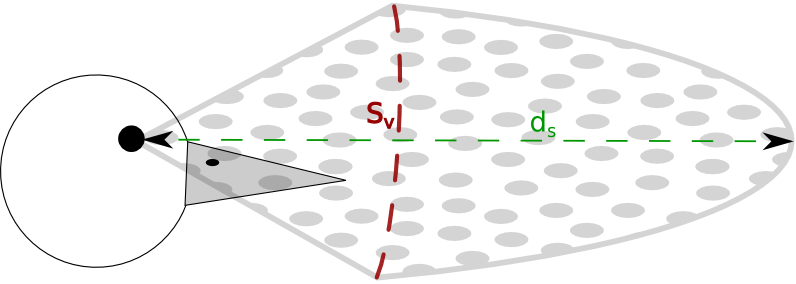
\includegraphics[scale=0.45]{./images/birdflocking/verticalFow.png}
	\caption{Birds vertical field of view. \(d_s\) and \(s_v\) represent the sight distance and the vertical perceptual span, respectively. }
	\label{fig:vFOV}
	
\end{figure}	

\begin{figure}[h!]
	\centering
	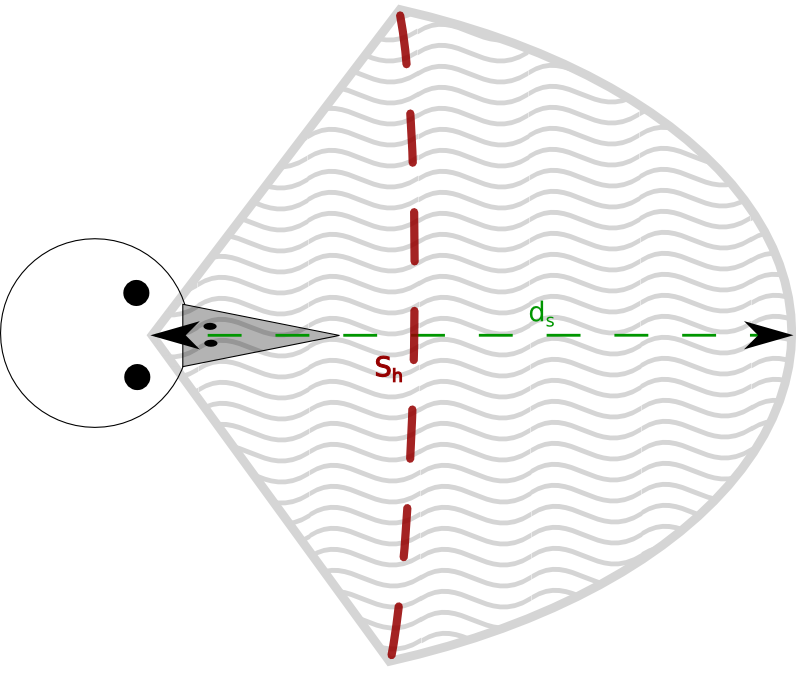
\includegraphics[scale=0.375]{./images/birdflocking/hFow.png}
	\caption{Birds horizontal field of view. \(s_h\) represents the horizontal perceptual span. \(d_s\) as in Fig. \ref{fig:vFOV}. }
	\label{fig:hFOV}
	
\end{figure}	


\subsection{Flight Model}
Bird $b$ flight at step $i$ is described by its $3$-dimensional space vectors
position $\vec{p}_b^i=\expval{p^i_x,p^i_y,p^i_z}$ and velocity
$\vec{v}_b^i=\expval{v^i_x,v^i_y,v^i_z}$, that correspond to its current sight
direction. 


The evolution of the bird's  velocity over time is regulated by
the following:
% * <spataro@unical.it> 2015-11-24T10:13:28.607Z:
%
% ^.
% * <spataro@unical.it> 2015-11-24T10:13:24.416Z:
%
% ^.

\begin{align}
\label{eq:birdCumulativeVelocities}
\vec{v}_b^{i+1} = (r sin\theta' cos \phi', \ r sin\theta' sin \phi', \ r cos \theta')
\end{align}

where:
\begin{itemize}
	\item $
	\theta' = \begin{cases}
	\theta_d &\mbox{ if }  |\theta_b - \theta_d| < \theta_{max}\\
	\theta_b + \theta_{max} &\mbox{ otherwise }\\
	\end{cases}
	$ \hfill \\
	\medskip
	\item $
	\phi' = \begin{cases}
	\phi_d &\mbox{ if }  |\phi_b - \phi_d| < \phi_{max}\\
	\\
	\phi_b + \phi_{max} &\mbox{otherwise, it should be adjusted}\\
	
	&\mbox{depending on the sign if it have to}\\
	&\mbox{go right or left}\\
	\end{cases}
	$ \hfill \\ 
	
	
	\item $ \vec{v}_d^i = \mu_c \vec{v}_c + \mu_s\vec{v}_s + \mu_a \vec{v}_a + \mu_{a} \left(
	\vec{{\tau}_i} + \vec{\Gamma}_i \right) + \vec{\omega}_i $
	
	\begin{itemize}
		\item $\mu_c$, $\mu_s$, $\mu_a$ are the cohesion, separation and alignment coefficient (social coefficients) and $\mu_a$ is the avoidance coefficient. 
	\end{itemize}
	\item  $\vec{v}^i_c$,$\vec{v}^i_s$, $\vec{v}^i_a$ are the  \textit{social velocities} \cite{Hemelrijk:2011}
	\begin{itemize}
		\item $\vec{v}^i_c$, the cohesion velocity that has direction parallel to the
		line that pass through $\vec{p}_b^i$ and the average position of its neighbors
		\item $\vec{v}^i_s$, the separation velocity, keep the bird at a minimum
		safety distance from its flockmates
		\item  $\vec{v}^i_c$, the align velocity, synchronize boids heading.
	\end{itemize}
	\item $\theta_d,\theta_b$ are the polar angle of the velocity vector
	$\vec{v}^i_b$ and $\vec{v}^i_d$ respectively.
	\item $\phi_d,\phi_b$ are the azimuthal angle of the velocity vector
	$\vec{v}^i_b$ and $\vec{v}^i_d$ respectively.
	
	
\end{itemize}


\subsection{Bird's Field of View}
Each bird has a limited visual capacity described by its field of view (FOV).
This implies that it can only perceive objects that are within its FOV. Bird
$o$'s FOV $\mathcal{F}_p$, is here defined as the set of points $p_n$ that
satisfy equations \ref{eq:fov1},\ref{eq:fov2} and \ref{eq:fov3}. An
object  $n$, in order to be within the  observer $o$'s neighbourhood,  must fall within
its viewing frustum i.e. the polar and azimuthal angle between observer's view
direction and the object should be less or equal than $s_h$ and $s_v$ respectively,
and the distance between them should be less than the maximum sight distance of the
observer $s_d$.
Let $\vb{p'_n}=\expval{p^x_n-v^x_o,p^y_n-v^y_o,p^z_n-v^z_o}$ the position vector of the object $n$ in the $o$'s frame of reference, then $n$ is $o$'s neighbor if and only if the followings hold:
\begin{equation}
\label{eq:fov1}
\delta_s = || \vb{p_o} - \vb{p_n} ||,\; \delta_s \leq d_s 
\end{equation}

\begin{equation}
\label{eq:fov2}
- \; \frac{s_h}{2} \leq \theta \leq \frac{s_h}{2}
\end{equation}

\begin{equation}
\label{eq:fov3}
- \; \frac{s_v}{2} \leq \phi \leq \frac{s_v}{2}
\end{equation}
where: 
\begin{align*}
&\phi = \arccos
\left(\frac{p'^z_n}{\sqrt{(p'^x_n)^2 + (p'^y_n)^2 + (p'^z_n)^2}}\right) \\
&\theta = atan2 \left(\frac{p'^y_n}{p'^x_n} \right) 
\end{align*}
We use the  two arguments $\tan$ version in order to gather information on the signs of the inputs in order to return the appropriate quadrant of the computed angle, which is not possible for the single argument $\arctan$ function. Additionally, the ordinary $\arctan$  suffers when required to produce  $\pm \frac{\pi}{2} $ angle \footnote{Computing angle between $x$ and $y$ axis would require a division by zero.}.
\begin{equation*}
\theta = 
\begin{cases}

\frac{\pi}{2},&\mbox{if }  p'^x_n=0, \ p'^y_n>0  \\

\frac{3\pi}{2},&\mbox{if } p'^x_n=0, \ p'^y_n<0 \\

\text{undefined} &\mbox{if } p'^x_n=0, p'^y_n =0 \\

\arctan \frac{p'^y_n}{p'^x_n} &\mbox{if } p'^x_n>0, \ p'^y_n \ge 0  \\

\arctan \frac{p'^y_n}{p'^x_n} + 2 \pi &\mbox{if } \ p'^x_n>0, \ p'^y_n < 0, \ \ or
\ p'^x_n<0, \ p'^y_n > 0 \\

\arctan \frac{p'^y_n}{p'^x_n} + \pi &\mbox{if }\ p'^x_n<0, \ p'^y_n \le 0 
\end{cases}
\end{equation*}


\begin{figure}
	\minipage{0.40\textwidth}
	\begin{subfigure}{1.0\textwidth}
		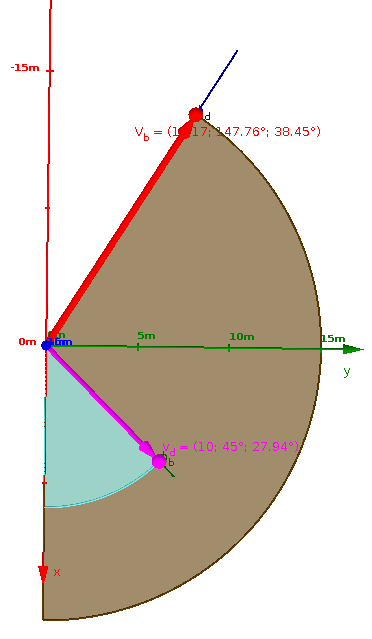
\includegraphics[width=\linewidth]{./images/birdflocking/horizonthal}
	
		
	\end{subfigure}		
	\endminipage\hfil
	\minipage{0.40\textwidth}
	\begin{subfigure}{1.0\textwidth}
		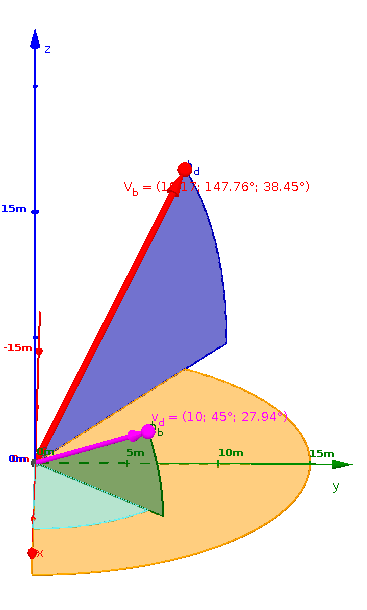
\includegraphics[width=\linewidth]{./images/birdflocking/vertical}
		
	\end{subfigure}
	\endminipage
	\caption{Example of spherical coordinate representation of two vectors. .$V_d$ for instance is a vector of magnitute 10 and polar and aximuthal angles 45° and 27.94° respectively.(a) and (b) show views from the top and from the side of the reference frame.}
\end{figure}


\subsection{Cohesion}
Cohesion is a flight behaviour that attracts a bird to centroid of  its perceived
neighbourhood. 
In formal terms \(\vec{C}_b^i\), the bird $b$'s centroid at time $i$, is given by:

\begin{align}
\vec{C}_b^i = \frac{1}{|\mathcal{N}_b|}\sum_{n=1}^{|\mathcal{N}_b|}{\vec{p}_n  \frac{d_{i,j}}{d_s}}
\end{align}

where:

\begin{enumerate}
	\item \(\mathcal{N}_b\) the set of birds in b's FOV.
	\item \(\vec{p}_n\) is the position of $n \in \mathcal{N}_b$
	\item \(d_{i,j}\) is the distance between bird \emph{b} and its neighbour
	\emph{c}
	
\end{enumerate}

The $b$'s cohesion vector \(\vec{v}_c\) is then defined as follows.

\begin{equation}
\vec{v}_c^i =
\begin{cases}
\frac{\vec{C}_b^i - \vec{p}_b}{|| \vec{C}_b^i - \vec{p}_b ||} +
a, &\mbox{ if } 0 < |\vec{v}_d| \leq v_p \\
v_p, &\mbox{ otherwise } 
\end{cases}
\end{equation}

\subsection{Separation}
\label{sect:separation}
A bird try to keep certain distance between itself and
its neighbors. Bird $b$'s separation velocity $\vec{S}_b^i$ at time $i$ is given
by:


\begin{equation}
\vec{S}_b^i = 
\begin{cases}
\left[\sum_{j \in \mathcal{N}_b}{\frac{\vec{p}_b -
		\vec{p}_j}{||\vec{p}_b - \vec{p}_j||}} \;f_s\right] + a ,&\mbox{if } 0 < |\vec{S}_i|
\leq v_p\\
v_p, &\mbox{ otherwise } 
\end{cases}
\end{equation}

where:

\begin{enumerate}
	\item \(\mathcal{N}_b\) is the set of neighbours, %the number of ,
	\item $
	f_s = \begin{cases}
	0 &\mbox{ if }  d_{i,j} > d_{min}\\
	1 - \frac{d_{i,j}}{d_{min}} &\mbox{ otherwise}
	\end{cases}$
\end{enumerate}

\subsection{Alignment}
A bird tries to match its velocity (speed and heading) with those of
nearby flockmates. This behaviour is called velocity alignment. Real life birds only consider a relatively small number flockmates while performing this behaviour and it usually is about seven neighbours\cite{Hemelrijk:2011}.
In formal terms, bird $b$'s alignment \(\vec{A}_b^i\) is here defined as %(equation \ref{eq:alignment})

\begin{align}
\vec{A}_i = \left[\sum_{j \in \mathcal{N}'_b}{\vec{v_j}}\;f_a\right] + a, \;\;0 < |\vec{A}_i| \leq v_p
\label{eq:alignment}
\end{align}

where:

\begin{enumerate}
	\item \(\mathcal{N}'_b \subseteq \mathcal{N}_b\) is the set of birds considered by $b$ for the alignment (e.g. the nearests).
	\item \(\vec{v}_j\) is the $j$'s velocity.
	\item \(f_a\) is the alignment coefficient. Let \(d_{i,j}\) the distance between bird \emph{i} and \emph{j} then \(f_a\) is given by:
	
	\begin{equation*}
	f_a = \begin{cases}
	0 &\text{, if $ d_{i,j} > d_a$}\\
	1- \frac{d_{i,j}}{d_a} &\text{, otherwise}
	\end{cases}
	\end{equation*}
\end{enumerate}

\subsection{Other species and predator avoidance}
\textsc{ACIADDRI} is a multi-agent with multiple group model where each group correspond to a different bird's species or to the group of predators. 
Different species interaction is described in section \ref{sect:otherSpecieAvoidance} and predator avoidance in section \ref{sect:predatorAvoidance}.

\begin{enumerate}
	\item \textbf{Other species avoidance}
	\label{sect:otherSpecieAvoidance}
	This behaviour is similar to \textit{separation} (see section \ref{sect:separation}) with the difference that a only birds from other species are taken into consideration. In formal terms the other specie avoidance vector  \(\vec{\tau}_i\) is given by:
	
	\begin{equation}
	\vec{\tau}_i = 
	\left[\sum_{j \in \mathcal{N}_b}{\frac{\vec{p}_b -\vec{p}_j}{||\vec{p}_b - \vec{p}_j||}} \;f_s\right] + a 
	\end{equation}
	where:
	
	\begin{enumerate}
		\item \(\mathcal{N}_b\) is the number of neighbours of specie different from the one of $b$,
		
		\item $
		f_s = \begin{cases}
		0 &\mbox{ if }  d_{i,j} > r_s\\
		1 - \frac{d_{i,j}}{r_s} &\mbox{ otherwise}
		\end{cases}$
	\end{enumerate}
	
	
	\item \textbf{Predator avoidance}
	\label{sect:predatorAvoidance}
	The predator avoidance vector is computed by taking in consideration position and velocity (speed and heading) of all the  predators within the bird's FOV. Intuitively birds will flee from the future (step $i+1$) centroid of predators's position \cite{Laird}. Formally the predator avoidance vector $\vec{\Gamma}_b^i$ is defined as follows:
	
	\begin{align}
	\vec{\Gamma}_b^i = \left[\sum_{j \in \mathcal{P}_b }{\frac{\vec{p}_i -
			(\vec{p}_j+\vec{v}_j)}{||\vec{p}_i - (\vec{p}_j+\vec{v}_j)||}} \;f_{p}\right] +
	a, \;\;0 < |\vec{\Gamma}_i| \leq v_p
	\end{align}
	
	where:
	
	\begin{enumerate}
		\item \(\mathcal{P}_b\) is the $b$'s set of predators
		\item $	f_{p} = \begin{cases}
		0 &\mbox{ if }  d_{i,j} > r_p\\
		1 - \frac{d_{i,j}}{r_p} & \mbox{ otherwise}
		\end{cases}
		$ \hfill \\
		is the predator avoidance coefficient.
	\end{enumerate}
\end{enumerate}

\subsection{Wandering}
When the neighbourhood  of a bird is empty it flies pseudo-randomly in the space. This kind of behaviour is called \textit{wandering}. 
Wandering is obtained combining a current and a random direction 
\begin{equation*}
\vec{\omega}_b^i =  
\begin{cases} 
0 &\mbox{if } \mathcal{N}_b \neq \emptyset \\ 
\frac{\vec{s}}{|\vec{s}|}\;w_r+w_d,\; 0 < |\vec{\omega}_i| \leq v_p & \mbox{otherwise }. 
\end{cases}
\end{equation*}


\lstset{frame=tb,
	basicstyle=\footnotesize\ttfamily,
	keywordstyle=\color{blue}\ttfamily,
	stringstyle=\color{red}\ttfamily,
	commentstyle=\color{green}\ttfamily,
	backgroundcolor=\color{light-gray}, 
	numbers=left,numbersep=3pt, 
	numberstyle=\tiny\ttfamily\color{gray}
	%	numberstyle=\tiny
}

\section{GPGPU Parallel implementation and Results}
\label{sect:gpuimplementation}
In this work we adopt GPUs and the CUDA framework to accelerate the flocking
simulation of a large number of boids using the the model presented in section
\ref{sect:aciaddri} in an environment with a number of agents up to $5
\times10^6$.
According to the APOD development methodology we produced two different parallel
versions, both sharing the high-level implementation structure that consists in
(the well-known host-managed accelerated program structure):
\begin{itemize}
	\item Initialization of data structures on \emph{CPU}
	\item Data transfer from \textbf{\emph{CPU} to \emph{GPU}}
	\item Kernels execution on \emph{GPU}
	\item Copying the result back from \textbf{\emph{GPU} to \emph{CPU}}
\end{itemize}
The parallelization strategy is designed with the purpose to avoid as much
as possible the very undesirable data copy from \emph{host to device}  , or vice versa\cite{CUDA3} \cite{Spataro} \cite{Dambrosio}.
The computation of $\vec{p}_b^{i+1}$ and $\vec{v}_b^{i+1}$ is entirely performed on GPU and implemented as composition of CUDA kernels. Moreover Parameters are stored in constant memory for fast access.
An OpenGL 3D visualization tool comes with the simulation system and permits real time and interactive 
rendering of the flocking model.

\subsection{Na\"{i}ve version}
In this version each agent is mapped to a CUDA thread organized in a 1D block-grid structure.
All data resides in global memory and user managed cache (shared memory) remains unused. 
Due to the high parallel nature of the simulation, although its simplicity, this version already gives rise to a speedup of $\approx20 \times$. In addition, an optimization was carried out by considering the \emph{If-Divergence mitigation}. As known, thread divergence is a well known
issue, that inhibits full parallelism at warp level. Two threads are said to
diverge if they belong to the same warp but execute different
instructions\footnote{Common code constructs that usually cause thread
	divergence are conditionals that depends on  thread-id variable}. If some
threads in a warp evaluate a conditional to \emph{true} and others to \emph{false}, then threads will branch to different instructions paths
and those paths are executed in \emph{serial manner}\footnote{It is important to
	stress that serial execution happens only when thread of the same warps 
	diverge.}\cite{NvidiaprogGuide}. As a consequence, this serialization may result in significant performance loss.

A series of workarounds have been implemented in order to mitigate this problem and more specifically, a number of $if$ construct have been substituted with an equivalent arithmetical operation that are performed by all threads and preserves the original semantic of the code. Listings \ref{list:divergent} and \ref{list:notDivergent} show an example of such code transformation.

\begin{lstlisting}[label={list:divergent}, caption={Example of thread divergent code.} ]
private var;
if(threadIdx.x > 16) then
var:= A
else
var:= B
\end{lstlisting}

\begin{lstlisting}[label={list:notDivergent}, caption=If mitigated version of the listing \ref{list:divergent} ]
bool c = threadIdx.x > N
private var;
var:= c*A + !c*B
\end{lstlisting}


\subsection{Shared memory version}
This version exploits the shared memory in order to cache birds's frequently accessed data. Shared memory is much faster than global memory but is of limited capacity (and depends on compute capability of the device, $48 KB$ in the \emph{GTX980})\cite{CUDA2}, only accessible at block level and cleared at each kernel invocation. This implies a number of restrictions on its usage, namely:

\begin{enumerate}
	\item it has to be initialized (i.e. requires a global memory access, see line 7 in listing \ref{list:sharedMemory}),
	\item limited size of data available per thread,
	\item cannot be used to share data between threads of different blocks.
\end{enumerate}
The adopted strategy divides the computation in a number of phases that depend on the chosen block size. Each phase can be then performed exploiting the fast memory as shown in listing \ref{list:sharedMemory}.
The above points 2 and 3 are the main reason for the division in phases.
Moreover the constraint posed by \textsc{aciaddri} that requires that each bird know about all the other birds (to decide if it falls within its FOV for instance) make impossible to load all the data in shared memory \cite{Richmond_ahigh,Nguyen:2007}.
\begin{lstlisting}[label = {list:sharedMemory}, caption=Main loop of the agent function kernel. The loop variable represents the number of phases which one at time use SM to store data of a portion of the whole bird population.]
extern __shared__ Bird shBird[];
uint loop = NBIRDS/BLOCK_X  + (NBIRDS % BLOCK_X ? 1 : 0);
#pragma unroll
for (uint i = 0; i < loop; i++) {
int idx = i * blockDim.x + threadIdx.x;
if(idx<NBIRDS)
shBird[threadIdx.x]=birds[idx];

...
COMPUTATION USING SM shBird
...

\end{lstlisting}

Three  devices were adopted for testing different CUDA version of the
model: the high-end GTX 980, a GT 635M and a low-end mobile chip (see
table \ref{tab:adoptedHW} for further details).

In order to ensure the correctness of the parallelization the output of each parallel version were matched against the corresponding serial output. In particular, the sequential CPU version is identical to the version that was developed for the GPUs, that is, no optimizations were adopted in the former version. In practice, at every step, the CA space array is scrolled and the transition function applied to each cell of the CA where bird is present.

\begin{table}[h!]
	\centering
	\begin{tabular}{|l |l |l| l|l|}
		\hline
		Name & Comp. Capability & RAM &
		SM-Clock & \# cores\\
		\hline
		GT 653M & \(2.1\) & \(1024\)MB  & $675$ MHz  & 635\\
		GTX 980& \(5.5\) & \(4096\)MB  & $1216$ MHz & 2048 \\
		TESLA K40& \(5.2\) & \(12288\)MB  & $875$ MHz & 2880 \\
		\hline
	\end{tabular}
	\caption{Hardware utilized for experiments}
	\label{tab:adoptedHW}
\end{table}

Different tests were carried out regarding both parallelizations described in the previous sections, and by considering different number of boids and an environment composed of $1000 \times 1000 \times 1000 $ cells. Each simulation was carried out for $10^4$ time steps. 

Tables \ref{tab:naive} and \ref{tab:ifdiv} shows the execution times of the na\"ive and shared memory version, respectively.
\begin{table} [h!]
	\centering
	\begin{tabular}{|l |l |l| l|}
		\hline
		\# birds & Sequential & GT	635M ($\times$) & GTX 980 ($\times$) 
		\\
		\hline
		
		1024  	& \(263.9\) 	& $29.1$, ($9,07$) 	& $10.5$, ($25,13$) \\
		5120  	& \(4913.0\) 	& $574.4$, ($8,55$) 	& $51.7$, ($95,02$)  \\
		10240 	&  $19074.5$ 	& $2241.6$, ($8.51$) 	& $109.0$, ($174,99$)  \\
		15360 	& \(43332.3\) 	& $5004.7$, ($8.65$) 	& $235.2$, ($184,23$)  \\
		20480  	& 86065.7 		& $8868.9$, ($9,70$) 	& $312.5$, ($275.408$) \\
		40960  	& 452423.1 		& - 						& $1023.8$, ($441.90$)  \\
		81920  	& 1966134.9 	& - 						& $3663.5$, ($536,70$)  \\
		163840  & 8003173.0 	& - 						& $14877.4$, ($537,94$)	 \\
		327680  & 35815012.0 	& - 						& $58003.0$, ($617,47$)  \\
		\hline
	\end{tabular}
	\caption{Timing (in seconds) for the Parallel CUDA Na\"ive implementation}
	\label{tab:naive}
\end{table}

\begin{table} [h!]
	\centering
	\begin{tabular}{|l |l |l| l|}
		\hline
		\# birds & Sequential & GT	635M & GTX 980
		\\
		\hline
		s
		1024  & \(263.9\) & $19.9$ & $7.9$  \\
		5120  & \(4913.0\) & $366.3$ & $34.6$  \\
		10240 &  $19074.5$ & 1398.7 & 96.5  \\
		15360  & \(43332.3\) & $3110.0$ & $154.9$  \\
		20480  & 86065.7 & 5522.0 & $280.8$ \\
		40960  & 452423.1 & - & $825.4$ \\
		81920  & 1966134.9 & - & $3307.2$ - \\
		163840  & 8003173.0 & - & $13565.9$ \\
		327680  & 35815012.0 & - & $54113.4$  \\
		\hline
	\end{tabular}
	\caption{Timing (in seconds) for the Parallel CUDA Na\"ive implementation}
	\label{tab:ifdiv}
\end{table}

Timings reported for the considered GPU devices indicate their full suitability for parallelizing multi-agent models, demonstrating the effectiveness of GPGPU to cut down computational time. In fact, the adoption of the CUDA technology has produced dramatic improvements in model speedup on the considered hardware up to 617x. 




\section{Conclusions and Future Outcomes}
\label{sect:Discussion}

Starting from Reynolds's behavioural model, we have here presented a preliminary multi-agent and multiple group approach for bird flocking, together with an efficient implementation by means of the CUDA framework. Experiments carried out by adopting different hardware have proven the full suitability of the GPGPU paradigm for efficiently simulating multi-agent systems.
Although our model describes bird movement adequately, future versions of \textsc{ACIADDRI} can take into account more behaviours by adding some parameters to improve the bird's flight modelling \cite{Dutta:2010,phys.org,Gangshan:2014} as the introduction of stall velocity (that represents the velocity's lower bound) or wing's length and width (for thrust and lift forces computation), to better adhere with aerodynamics theory. 

In current \textsc{ACIADDRI} implementation, all the computational intensive computations are carried out on the device and only final results are sent back to the host.
When the proper mode is active, data is transferred from GPU to CPU at fixed times steps for visualization purposes.
This results in additional time costs related to both the transfer and rendering on CPU.
In order to avoid this issue, the adoption of OpenGL / CUDA interoperability will be investigated, permitting to directly and effectively copy data from device memory to the GPU display buffer to avoid the aforementioned additional costs, resulting in an more efficient solution.

Eventually, future developments will also regard model improvement, such as the possibility of the environment to contain obstacles, and the usage of multi-gpu hardware \cite{Kirk2010,Cheng:2014}, which can further scale the performance of the application and dramatically speed up the overall simulation process.
